\documentclass[12pt]{article}
\usepackage[margin=1in]{geometry}
\usepackage[UTF8]{ctex}
\usepackage{amsmath, amsfonts, amssymb}
\usepackage{graphicx}
\graphicspath{{./images/}}
\usepackage{hyperref}
\usepackage{color}
\usepackage{multirow}
\usepackage{booktabs}   
\usepackage{adjustbox}
\usepackage[
backend=biber,
style=alphabetic,
]{biblatex}
\usepackage[english]{babel}
\addbibresource{references.bib}

% Define red alert TODO
\newcommand{\todo}[1]{\textcolor{red}{TODO: #1}}

\title{V2}
\author{Chunyu Yang}
\date{\today}

\begin{document}
\maketitle

\section{System Model}
\label{sec:system_model}

We consider an interference scenario where geostationary orbit (GSO) satellites serve as primary communication nodes while low Earth orbit (LEO) satellites from non-geostationary systems act as potential interference sources. The core analysis focuses on downlink transmissions observed at a GSO ground station (GGS), where the composite received signal contains both desired GSO carrier waves and unintended LEO interference components, as illustrated in Fig.~\ref{fig:interference-scenario}.

\subsection{Link Budget Fundamentals}
The foundation of our modeling approach lies in comparative link budget analysis. For the desired GSO signal, the received carrier power is determined through classical satellite communication relationships:

\begin{equation}
    C = \frac{\text{EIRP}_{\text{gso}} \cdot G_{\text{r, gso}}(\theta_0)}{L_{\text{FS, gso}} \cdot L_{\text{add}}}
\end{equation}

where $G_{\text{r, gso}}(\theta_0)$ represents the maximum receive antenna gain aligned with the GSO's boresight angle $\theta_0$, while $L_{\text{FS, gso}}$ and $L_{\text{add}}$ account for free-space propagation loss and aggregate atmospheric impairments, respectively.

Interfering contributions from LEO satellites introduce several spatial-temporal complexities. Each $k$-th LEO interferer contributes a distinct power component:

\begin{equation}
    I_k = \frac{\text{EIRP}_k \cdot G_{\text{r, k}}(\theta_k) \cdot B_{\text{adj, k}}}{L_{\text{FS, k}} \cdot L_{\text{add}}}
\end{equation}

Here, the angular dependence $G_{\text{r, k}}(\theta_k)$ reflects the dynamic geometric relationships between rapidly moving LEO satellites and the fixed GGS location. The bandwidth overlap factor $B_{\text{adj, k}} \in [0,1]$ modulates interference severity based on spectral alignment between GSO and LEO transmissions.

The combined signal quality metric is expressed through the carrier-to-interference-plus-noise ratio:

\begin{equation}
    \text{CINR} = \frac{C}{\sum_{k=1}^{K}I_k + k_{\text{B}}TB}
\end{equation}

where $k_{\text{B}}$ denotes the Boltzmann constant, $T$ the system noise temperature, and $B$ the operational bandwidth. This formulation encapsulates the thermodynamic noise floor along with aggregate interference from $K$ co-channel LEO satellites.

\subsection{Composite Signal Characterization}
The physical-layer received signal at the GGS integrates three fundamental components:

\begin{equation}
    y(t) = \underbrace{x(t)\sqrt{\text{CNR}}}_{\text{Desired GSO}} + \underbrace{\sum_{k=1}^{K} i_k(t)e^{j2\pi \Delta f_k t}\sqrt{\text{INR}_k}}_{\text{LEO interference}} + \underbrace{\zeta(t)}_{\text{Noise}}
\end{equation}

Here, $\Delta f_k = f_{\text{c},k} - f_{\text{c,gso}}$ captures carrier frequency offsets arising from orbital dynamics and Doppler effects. The quadrature terms $e^{j2\pi\Delta f_k t}$ induce time-varying phase rotations determined by each LEO satellite's orbital trajectory and transponder characteristics.

To support subsequent machine learning processing, we derive dual-domain representations of the received signal. The time-domain representation $y^A$ consists of uniform amplitude samples capturing instantaneous signal behavior. Frequency-domain characterization employs Welch's power spectral density (PSD) estimation, producing logarithmic magnitude spectra through overlapping windowed transforms: $y^F = 10\log_{10}(\phi(y(t)))$. This PSD representation effectively captures long-term spectral occupancy patterns crucial for interference analysis.


\section{Proposed Deep Learning Model}

\subsection{Mutual Attention Fusion}
\label{subsec:fusion}

Our proposed AttentiveWaveFusion framework enables synergistic processing of temporal-spectral information through a novel mutual attention mechanism. As illustrated in \autoref{fig:architecture}, the system comprises two fundamental stages: (1) parallel signal decomposition through dedicated encoding pathways, and (2) cross-domain feature interaction via bidirectional attention fusion.


The input signal first undergoes multi-modal decomposition through separate convolutional encoders:
\begin{equation}
    \begin{aligned}
        \mathbf{H}_t & = \text{TimeEncoder}(X_t) \in \mathbb{R}^{B \times 64 \times L}, \\
        \mathbf{H}_f & = \text{FreqEncoder}(X_f) \in \mathbb{R}^{B \times 64 \times L},
    \end{aligned}
\end{equation}
where $X_t$ and $X_f$ represent the raw temporal waveform and its wavelet coefficients respectively. Each branch employs 1D convolutions with stride 2 for dimension reduction and channel expansion ($C=64$), extracting complementary signal characteristics in their respective domains.


Rather than naive concatenation, our architecture implements bidirectional cross-attention to establish dynamic time-frequency correlations. Given encoded features $\mathbf{H}_t$ and $\mathbf{H}_f$, we compute the mutually enhanced representations:

\begin{equation}
    \begin{aligned}
        \mathbf{H}_t' & = \text{MutualAttn}_t(\mathbf{H}_t, \mathbf{H}_f) + \gamma_t \mathbf{H}_t, \\
        \mathbf{H}_f' & = \text{MutualAttn}_f(\mathbf{H}_f, \mathbf{H}_t) + \gamma_f \mathbf{H}_f,
    \end{aligned}
\end{equation}

where $\gamma_{(\cdot)}$ are learnable scaling parameters initialized to 0. The mutual attention operator $\text{MutualAttn}(x,y)$ implements:

\begin{equation}
    \text{Attention}(x,y) = \text{Softmax}\left(\frac{(\mathbf{W}_Q x)^\top (\mathbf{W}_K y)}{\sqrt{d}}\right)(\mathbf{W}_V y),
\end{equation}

\noindent with learnable projections $\mathbf{W}_{Q/K/V} \in \mathbb{R}^{64 \times 64}$ shared across domains. The L×L affinity matrix encodes pairwise temporal correlations by computing dot-products between all time steps' Q (from $x$) and K (from $y$) vectors.

% \begin{figure}[t]
%     \centering
%     \includegraphics[width=0.9\linewidth]{att-fusion.pdf} 
%     \caption{Mutual attention workflow: (a) Temporal branch queries using spectral keys/values, (b) Spectral branch subsequently queries using temporal keys/values. The diamond operator denotes parameter sharing.}
%     \label{fig:mutual_attn}
% \end{figure}


Query, key and value matrices are reused across domains to reduce model complexity while reusing latent space alignment. This architecture adjusts to varying frequency resolution demands through content-adaptive weighting, ensuring robustness across diverse signal regimes.


\subsection{Wavelet Transformation Loss}

Our proposed architecture introduces a frequency-aware objective function through wavelet-domain regularization. The composite loss function consists of two complementary components:

\begin{equation}
    \mathcal{L}_{\text{total}} = \mathcal{L}_{\text{MSE}} + \lambda\mathcal{L}_{\text{Wavelet}}
    \label{eq:combined_loss}
\end{equation}

where $\mathcal{L}_{\text{MSE}}$ denotes the conventional mean squared error in the time domain, and $\mathcal{L}_{\text{Wavelet}}$ represents our spectral regularization term weighted by $\lambda=0.5$.


The wavelet transformation employs preset scale factors $\mathbf{S} = [s_1, s_2, ..., s_n]$ to generate analytic filters spanning distinct frequency bands. Each wavelet kernel $\psi_s(t)$ follows the modulated Gaussian form:

\begin{equation}
    \psi_s(t) = \cos\left(\frac{7}{4}\frac{t}{s}\right) \cdot \exp\left(-\frac{t^2}{2s^2}\right)
    \label{eq:wavelet_def}
\end{equation}

where $s \in \mathbf{S}$ determines the temporal support and center frequency (see \autoref{fig:wavelet_scales}). The filter bank contains $|\mathbf{S}|$ orthogonal bases normalized to unit energy.


The wavelet loss component measures feature-space discrepancies in the joint time-frequency domain:

\begin{equation}
    \mathcal{L}_{\text{Wavelet}} = \frac{1}{N}\sum_{i=1}^{N} \left\lVert \mathcal{W}(x_i) - \mathcal{W}(\hat{x}_i) \right\rVert_2^2
    \label{eq:wavelet_loss}
\end{equation}

where $\mathcal{W}(\cdot)$ denotes the multi-scale wavelet transform operator mapping inputs to $|\mathbf{S}|$ decomposition coefficients. Crucially, the scale factors $\mathbf{S}$ remain fixed during optimization to maintain stable frequency band analysis.



\begin{figure}[t]
    \centering
    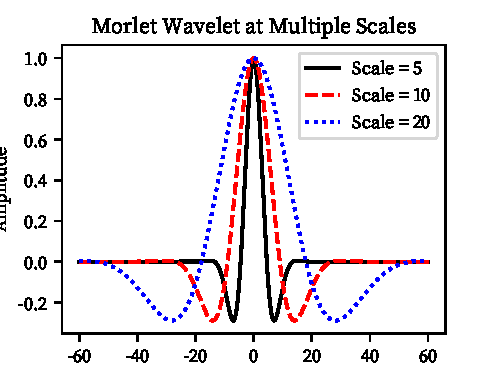
\includegraphics[width=0.5\linewidth]{wavelet-scales.pdf}
    \caption{Morlet-style wavelet kernels at different scales (\autoref{eq:wavelet_def}). Narrower windows (left) resolve high-frequency components while wider kernels (right) capture low-frequency structures.}
    \label{fig:wavelet_scales}
\end{figure}

\section{Experiments}

\subsection{Dataset Generation \& Characteristics}
\label{sec:dataset}

The synthetic dataset captures Ku-band (10.7-12.7 GHz) satellite interference scenarios through a 48-hour MATLAB simulation with 10-second sampling intervals, yielding 17,281 temporal snapshots. Each data sample comprises two synchronized representations: an 800-point time-domain waveform capturing instantaneous signal values and an 800-bin frequency-domain spectrum derived from Fourier transforms.

Binary labels identify interference presence, with class 0 denoting non-interference (aggregated interference-to-noise ratio (INR) below a predefined system protection threshold) and class 1 indicating substantial interference (INR exceeding this operational threshold). Labels derive from dynamic link budget calculations that account for time-varying channel conditions and satellite visibility patterns.

Instance-wise standardization normalizes both signal domains independently using per-sample mean (\( \mu \)) and standard deviation (\( \sigma \)) computed across the 800 measurement points:

\begin{equation}
    \hat{x}_i = \frac{x_i - \mu}{\sigma}
\end{equation}

To accomodate the anomaly detection task form, the training (11509 samples) and validation (1302 samples) sets contain exclusively non-interference data (class 0). The test set adopts a challenging real-world evaluation paradigm with 4470 samples divided into approximately balanced proportions: 2235 non-interference cases and 2235 interference scenarios. This split forces models to recognize interference signatures without prior exposure during training, mimicking actual deployment conditions where interference detection systems must identify novel anomalies.

The simulation accounts for adaptive coding/modulation through time-varying link losses (0-9 dB range) and generates extreme interference cases with peak aggregate INR reaching 32.47 dB, while background CNR fluctuates between 6.40 dB and 15.40 dB based on channel adaptations.

\subsection{Evaluation Results}

\begin{table}[htbp]
    \caption{Performance Comparison of DualAttnNet Against Baseline Models}
    \label{tab:main_results}
    \centering
    \begin{tabular}{lcccc}
        \toprule
        \textbf{Model} & \textbf{Accuracy (\%) } $\uparrow$ & \textbf{F1 Score} $\uparrow$ & \textbf{AUC}$\uparrow$ & \textbf{FLOPS (G)}$\downarrow$ \\
        \midrule
        DualAttnNet    & 0.8210                             & 0.8192                       & 0.9327                 & 0.00                           \\
        \cmidrule{1-5}
        LinearAE       & 0.7987                             & 0.7966                       & 0.9176                 & 0.00                           \\
        CNNAE          & 0.7996                             & 0.7975                       & 0.9175                 & 0.00                           \\
        Transformer AE & 0.5678                             & 0.5634                       & 0.6812                 & 0.00                           \\
        \bottomrule
    \end{tabular}
\end{table}


\subsection{Abalaton study}

\begin{table}[htbp]
    \caption{Ablation Study of DualAttnNet Components}
    \label{tab:ablation}
    \centering
    \begin{tabular}{lccc}
        \toprule
        \textbf{Model Variant} & \textbf{Accuracy (\%)} $\uparrow$ & \textbf{F1 Score} $\uparrow$ & \textbf{AUC} $\uparrow$        \\
        \midrule
        DualAttnNet (Full)     & 0.00                              & 0.00                         & 0.00                           \\
        \cmidrule{1-4}
        w/o Mutual Attention   & 0.00                              & 0.00                         & 0.00                           \\
        w/o Wavelet Loss       & 0.00                              & 0.00                         & 0.00                           \\
        Vanilla Implementation & 0.00                              & 0.00                         & 0.00                           \\
        \bottomrule
    \end{tabular}
    \vspace{2pt}

\end{table}



\end{document}